\chapter{Die Eclipse Plattform}
\label{chap:platform}

In diesem Kapitel wird gezeigt, welche Möglichkeiten Eclipse bietet, eine moderne Entwicklungsumgebung zu implementieren. Die Möglichkeiten werden miteinander verglichen und die Vor- und Nachteile aufgezeigt. Auch werden die wichtigsten Eclipse-Features, die für das Entwickeln von Applikationen auf der Eclipse Rich Client Platform (RCP) benötigt werden, beschrieben.

\section{Die Plattform}

Eclipse RCP bietet eine Basis, um betriebssystemunabhängige Applikationen zu entwickeln. Es bietet Mechanismen wie Plugins und Extension Points, um modulares Programmieren zu unterstützen und zu vereinfachen. Auch bietet das Framework Features wie Views, Editoren und Perspektiven, die häufig in Applikationen gebraucht werden.

\section{Plugins}

Eclipse-Applikationen nützen eine auf der OSGi Speizifikation basierten Laufzeitumgebung. Eine Komponente in dieser Umgebung ist ein Plugin. Eine Eclipse-RCP-Applikation besteht aus einer Ansammlung solcher Plugins.\cite{whatisaplugin} Plugins haben einen Lebenszyklus und können zur Laufzeit geladen oder entfernt werden. Ein Eclipse-Plugin kann Extension Points anderer Plugins nutzten und eigene Extension Points oder APIs anbieten.

\section{Extension Points}
\label{extensionpointssection}

Um Plugins erweitern zu können, bietet Eclipse das Konzept der Extension Points an. Über Extension Points können Plugins eine bestimmte Funktionalität anbieten, die von anderen Plugins verwendet werden kann. 
\newline
Eclipse bietet zum Beispiel ein Plugin an, das einen Extension Point für Views definiert. Andere Plugins können über diesen Extension Point, eine neue View erstellen und diese konfigurieren. \cite{extensionpoints}

\newpage
Die Abbildung \ref{fig:extensionpoint} zeigt, wie über diesen Extension Point eine neue Eclipse View erstellt werden kann.
\begin{figure}[H]
	\centering
		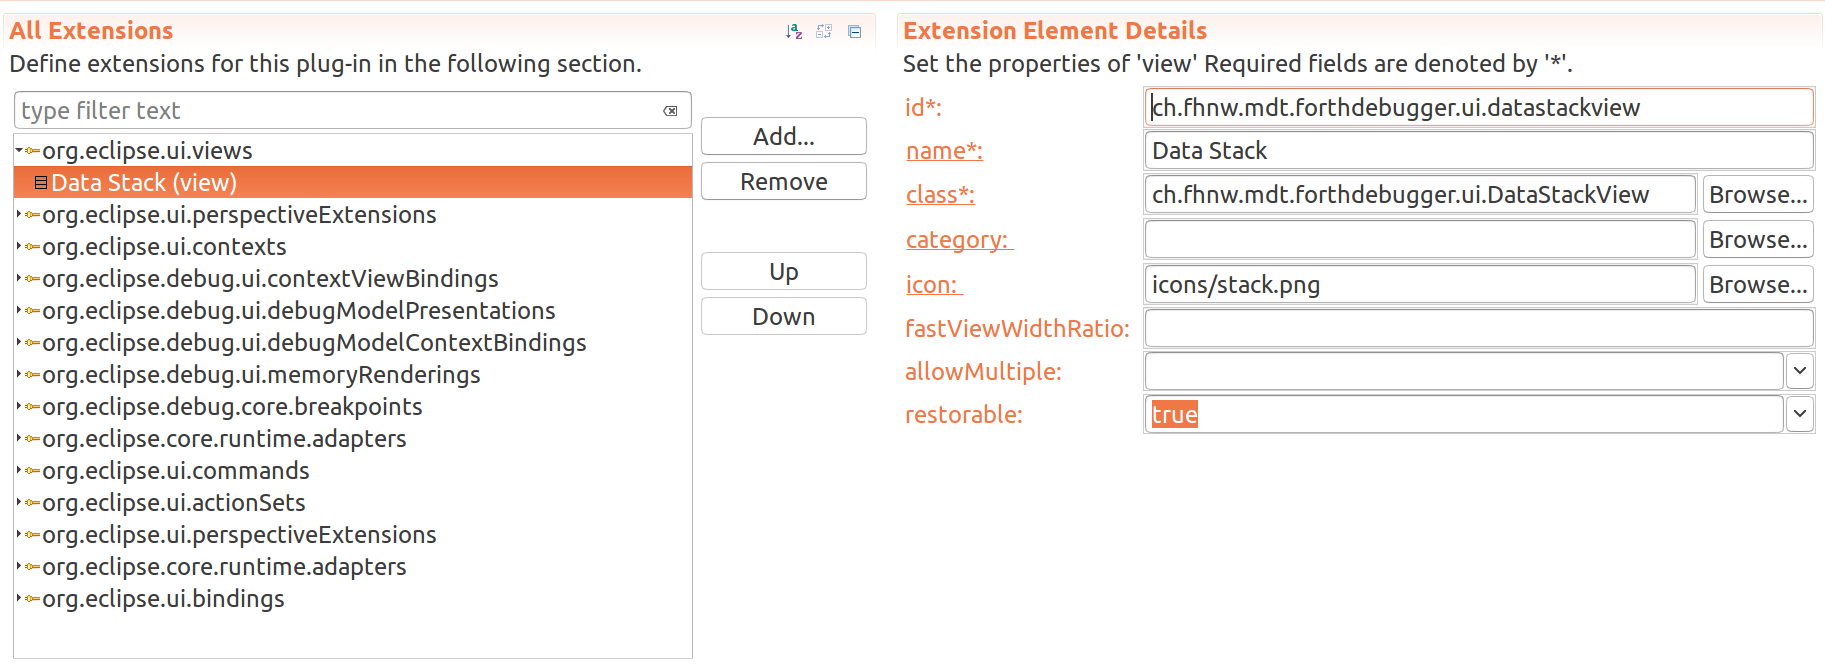
\includegraphics[scale=0.25]{platform/extensionpoint2.png}
		\caption{Ein Plugin, das einen Extension Point anbietet. Andere Plugins können diese deklarativ in einem XML File ansteuern.}
		\captionsetup{margin=0cm,font={footnotesize}}
		\label{fig:extensionpoint}
\end{figure}

Es ist auch möglich, eigene Extension Points zu definieren, falls ein Plugin anderen Entwickler für Erweiterungen offen stehen soll.

\section{Eclipse basierte MCore Entwicklungsumgebung}

Eclipse eignet sich besonders gut als Grundlage für eine Entwicklungsumgebung, da es schon einiges an Funktionalität für eine Entwicklungsumgebung zur Verfügung stellt und schon viele Entwicklungsumgebungen (PHP, C/C++, Python, D u.a.) basierend auf Eclipse entwickelt wurden. Auch existieren einige Tools, auf welche ich noch genauer eingehen werde, wie Xtext und DLTK, die das Programmieren einer Entwicklungsumgebung weiter vereinfachen. In den folgenden Kapiteln wird kurz auf die Möglichkeiten, wie die von Eclipse bereitgestellten Technologien verwendet werden könnten, eingegangen.

\subsection{JDT}
Um die MCore-Entwicklungsumgebung zu implementieren, könnten die Standard Features von dem Eclipse Java Development Tools (JDT) verwenden werden. Dies wäre sehr aufwändig, da alle Features für C (wie Syntax Highlighting, Code Completion oder eine Outline) neu implementiert werden müssten.

\subsection{Xtext}
XText ist ein Framework, das das Programmieren einer auf Eclipse basierten Entwicklungsumgebungen erleichtert. Es ermöglicht, auf schnelle Art und Weise das Grundgerüst einer Entwicklungsumgebung mit folgenden Features zu generieren:\cite{xtext}

\begin{itemize} 
	\item Editor mit Syntax Coloring
	\item Code Completion
	\item Compiler Integration
	\item Java-basierter Debugger
	\item Outline
	\item Indexing
\end{itemize}

Es muss lediglich eine ANTLR-ähnliche Grammatik für die Sprache definiert werden.\cite{antlr} Eine Grammatik für den C-Editor zu definieren ist schwierig. Ausserdem müsste noch der Präprozessor mit einbezogen werden, was Xtext standardmässig nicht unterstützt. \newline Für den Forth-Editor ist es aber durchaus möglich, Xtext zu verwenden. Im Kapitel "`\nameref{chap:fortheditor}"' wird beschrieben, wie Xtext verwendet wurde, um einen Forth-Editor zu implementieren.

\subsection{Dynamic Language Toolkit Framework}
Das Dynamic Language Toolkit (DLTK) ist ein weiteres Framework, das das Grundgerüst für eine Entwicklungsumgebung generieren kann. Ursprünglich war das Framework nur für dynamische Sprachen geeignet, es kann aber auch für statische Sprachen verwendet werden. Die D-Entwicklungsumgebung wurde mit dem DLTK realisiert\cite{ddt}. Es bestehen aber dieselben Nachteile wie bei Xtext. Da C schwierig zu parsen ist, müsste trotz dem Framework noch viel implementiert werden. Die Sprache D verwendet keinen Präprozessor, deshalb konnte für diese Entwicklungsumgebung das DLTK Framework verwendet werden.

\subsection{Eclipse C/C++ Development Tools}
Eclipse C/C++ Development Tools (CDT) ist eine Eclipse Distribution mit Unterstützung für C und C++. CDT bietet viele Features für C, die schon vom JDT bekannt sind und stellt Extension Points zur Verfügung, um diese zu verwenden. So kann mit relativ wenig Aufwand ein neuer Compiler in die Entwicklungsumgebung eingebunden werden. Dies wurde auch schon mehrfach gebraucht, um verschiedene C/C++ Compiler in Eclipse CDT zu integrieren. Auf die Einbindung des Compilers wird im Kapitel \ref{chap:compilerintegration} genauer eingegangen.

\subsection{Verwendung für uCore Eclipse}
Ich habe mich dazu entschieden, das Eclipse CDT als Target-Plattform zu wählen. Somit können alle Features vom Eclipse CDT verwendet werden. Xtext wird zusätzlich verwendet, um den uForth-Editor zu implementieren.
